% ==============================================================================
% BỘ ĐỀ THAM KHẢO TUYỂN SINH 10 NĂM HỌC 2026-2027 SỞ GD&ĐT TP.HCM
% ĐỢT 9: CỤM 6 - ĐỀ 3 & CỤM 7 - ĐỀ 1 (14 CÂU TỰ LUẬN)
% ==============================================================================

% ==============================================================================
% CỤM 6 - ĐỀ THAM KHẢO 3 (Đề số 18)
% ==============================================================================

\begin{bt}%[9D6H18-2]
% nguon: Đề tham khảo Tuyển sinh 10 năm học 2026-2027 Sở GD&ĐT TP.HCM - Cụm 6 Đề 3, Bài 1
	Cho hàm số $(P)\colon y = \dfrac{2}{3}x^2$.
	\begin{enumerate}[a)]
		\item Vẽ đồ thị $(P)$ trên mặt phẳng tọa độ $Oxy$.
		\item Tìm điểm thuộc $(P)$ sao cho hoành độ khác $0$ và gấp $2$ lần tung độ.
	\end{enumerate}
	\loigiai{
		\begin{enumerate}[a)]
			\item Bảng giá trị tương ứng giữa $x$ và $y$ của parabol $(P)\colon y = \dfrac{2}{3}x^2$:
			\begin{center}
				\begin{tabular}{|c|c|c|c|c|c|}
					\hline
					$x$ & $-3$ & $-1{,}5$ & $0$ & $1{,}5$ & $3$ \\
					\hline
					$y = \dfrac{2}{3}x^2$ & $6$ & $1{,}5$ & $0$ & $1{,}5$ & $6$ \\
					\hline
				\end{tabular}
			\end{center}
			Đồ thị $(P)$ là một parabol đi qua gốc tọa độ $O(0;0)$, nằm phía trên trục hoành và nhận trục tung $Oy$ làm trục đối xứng.
			\begin{center}
				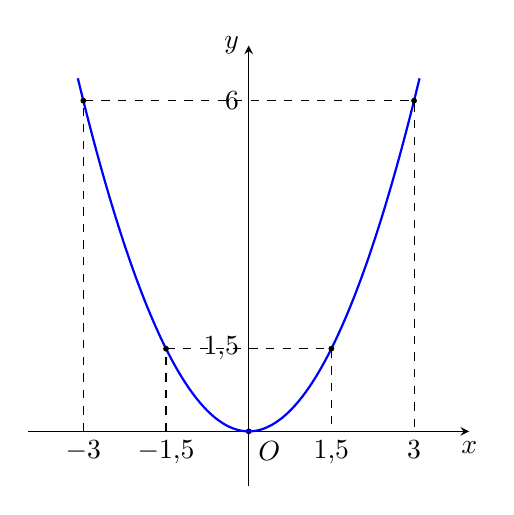
\begin{tikzpicture}[>=stealth, scale=0.7]
					\draw[->] (-4,0) -- (4,0) node[below] {$x$};
					\draw[->] (0,-1) -- (0,7) node[left] {$y$};
					\fill (0,0) circle (1.5pt) node[below right] {$O$};
					\draw[smooth, samples=100, domain=-3.1:3.1, thick, color=blue] plot(\x, {2/3*(\x)^2});
					\draw[dashed] (-3,0) node[below] {$-3$} -- (-3,6) -- (0,6) node[left] {$6$} -- (3,6) -- (3,0) node[below] {$3$};
					\draw[dashed] (-1.5,0) node[below] {$-1{,}5$} -- (-1.5,1.5) -- (0,1.5) node[left] {$1{,}5$} -- (1.5,1.5) -- (1.5,0) node[below] {$1{,}5$};
					\fill (-3,6) circle (1.5pt) (3,6) circle (1.5pt) (-1.5,1.5) circle (1.5pt) (1.5,1.5) circle (1.5pt);
				\end{tikzpicture}
			\end{center}
			\item Gọi tọa độ điểm cần tìm là $M(x; y) \in (P)$.
			
			Vì hoành độ gấp $2$ lần tung độ nên $x = 2y \iff y = \dfrac{1}{2}x$.
			
			Mặt khác $M \in (P)$ nên ta có phương trình:
			$$\dfrac{2}{3}x^2 = \dfrac{1}{2}x \iff \dfrac{2}{3}x^2 - \dfrac{1}{2}x = 0 \iff x\left(\dfrac{2}{3}x - \dfrac{1}{2}\right) = 0 \iff \left[\begin{aligned} &x = 0 \\ &x = \dfrac{3}{4}. \end{aligned}\right.$$
			Vì hoành độ khác $0$ nên $x = \dfrac{3}{4}$.
			
			Với $x = \dfrac{3}{4} \implies y = \dfrac{1}{2} \cdot \dfrac{3}{4} = \dfrac{3}{8}$.
			
			Vậy tọa độ điểm cần tìm là $\left(\dfrac{3}{4}; \dfrac{3}{8}\right)$.
		\end{enumerate}
	}
\end{bt}

\begin{bt}%[9D6H20-2]
% nguon: Đề tham khảo Tuyển sinh 10 năm học 2026-2027 Sở GD&ĐT TP.HCM - Cụm 6 Đề 3, Bài 2
	Cho phương trình $3x^2 - 9x + 4 = 0$.
	\begin{enumerate}[a)]
		\item Chứng minh phương trình luôn có hai nghiệm phân biệt $x_1, x_2$.
		\item Không giải phương trình, hãy tính giá trị của các biểu thức:
		$$A = x_1(x_1 - 3x_2) + x_2^2 + 2x_1 x_2 \quad\text{và}\quad B = x_1^3 + x_2^3.$$
	\end{enumerate}
	\loigiai{
		\begin{enumerate}[a)]
			\item Phương trình $3x^2 - 9x + 4 = 0$ có $a = 3, b = -9, c = 4$.
			
			Ta có:
			$$\Delta = b^2 - 4ac = (-9)^2 - 4 \cdot 3 \cdot 4 = 81 - 48 = 33 > 0.$$
			Vì $\Delta > 0$ nên phương trình luôn có hai nghiệm phân biệt $x_1, x_2$.
			\item Theo định lí Viète, ta có:
			$$\begin{cases} x_1 + x_2 = -\dfrac{b}{a} = 3 \\ x_1 x_2 = \dfrac{c}{a} = \dfrac{4}{3}. \end{cases}$$
			Ta tính:
			$$x_1^2 + x_2^2 = (x_1 + x_2)^2 - 2x_1 x_2 = 3^2 - 2 \cdot \dfrac{4}{3} = 9 - \dfrac{8}{3} = \dfrac{19}{3}.$$
			Biến đổi và tính biểu thức $A$:
			$$A = x_1^2 - 3x_1 x_2 + x_2^2 + 2x_1 x_2 = (x_1^2 + x_2^2) - x_1 x_2 = \dfrac{19}{3} - \dfrac{4}{3} = \dfrac{15}{3} = 5.$$
			Biến đổi và tính biểu thức $B$:
			$$B = x_1^3 + x_2^3 = (x_1 + x_2)(x_1^2 - x_1 x_2 + x_2^2) = (x_1 + x_2)\left[(x_1^2 + x_2^2) - x_1 x_2\right] = 3 \cdot \left(\dfrac{19}{3} - \dfrac{4}{3}\right) = 3 \cdot 5 = 15.$$
			Vậy $A = 5$ và $B = 15$.
		\end{enumerate}
	}
\end{bt}

\begin{bt}%[9D8H26-3]
% nguon: Đề tham khảo Tuyển sinh 10 năm học 2026-2027 Sở GD&ĐT TP.HCM - Cụm 6 Đề 3, Bài 3
	Biểu đồ dưới đây biểu diễn số học sinh ở mỗi tổ của lớp 9A trường THCS Hoàng Văn Thụ theo giới tính Nam và Nữ:
	\begin{center}
		\begin{tabular}{|l|c|c|c|c|}
			\hline
			\textbf{Tổ} & Tổ 1 & Tổ 2 & Tổ 3 & Tổ 4 \\
			\hline
			\textbf{Số học sinh nam} & 4 & 6 & 6 & 5 \\
			\hline
			\textbf{Số học sinh nữ} & 5 & 4 & 5 & 6 \\
			\hline
		\end{tabular}
	\end{center}
	\begin{enumerate}[a)]
		\item Hãy lập bảng tần số thống kê tổng số học sinh ở mỗi tổ của lớp 9A và cho biết lớp 9A có bao nhiêu học sinh.
		\item Giáo viên chủ nhiệm chọn ngẫu nhiên một học sinh của lớp 9A tham gia đội hình rước đuốc. Tính xác suất của các biến cố sau (dưới dạng phân số tối giản):
		\begin{itemize}
			\item Biến cố $A$: ``Học sinh được chọn thuộc tổ 1''.
			\item Biến cố $B$: ``Học sinh được chọn là học sinh nữ thuộc tổ 3 hoặc tổ 4''.
		\end{itemize}
	\end{enumerate}
	\loigiai{
		\begin{enumerate}[a)]
			\item Bảng thống kê số học sinh của mỗi tổ:
			\begin{center}
				\begin{tabular}{|l|c|c|c|c|c|}
					\hline
					\textbf{Tổ} & Tổ 1 & Tổ 2 & Tổ 3 & Tổ 4 & \textbf{Cả lớp} \\
					\hline
					\textbf{Số học sinh} & $4 + 5 = 9$ & $6 + 4 = 10$ & $6 + 5 = 11$ & $5 + 6 = 11$ & $41$ \\
					\hline
				\end{tabular}
			\end{center}
			Tổng số học sinh của lớp 9A là:
			$$9 + 10 + 11 + 11 = 41\text{ (học sinh)}.$$
			\item Không gian mẫu có số phần tử là $n(\Omega) = 41$.
			\begin{itemize}
				\item Biến cố $A$: ``Học sinh được chọn thuộc tổ 1''.
				
				Số học sinh thuộc tổ 1 là $9$ học sinh, nên số kết quả thuận lợi cho $A$ là $n(A) = 9$.
				
				Xác suất của biến cố $A$ là:
				$$P(A) = \dfrac{n(A)}{n(\Omega)} = \dfrac{9}{41}.$$
				\item Biến cố $B$: ``Học sinh được chọn là học sinh nữ thuộc tổ 3 hoặc tổ 4''.
				
				Số học sinh nữ thuộc tổ 3 là $5$, số học sinh nữ thuộc tổ 4 là $6$.
				
				Số kết quả thuận lợi cho biến cố $B$ là $n(B) = 5 + 6 = 11$.
				
				Xác suất của biến cố $B$ là:
				$$P(B) = \dfrac{n(B)}{n(\Omega)} = \dfrac{11}{41}.$$
			\end{itemize}
		\end{enumerate}
	}
\end{bt}

\begin{bt}%[9D6V21-3]
% nguon: Đề tham khảo Tuyển sinh 10 năm học 2026-2027 Sở GD&ĐT TP.HCM - Cụm 6 Đề 3, Bài 4
	Một nhóm tình nguyện viên muốn xây dựng một bể chứa nước sạch tạm thời có dạng hình hộp chữ nhật với chiều cao $2\text{ m}$. Đáy bể là hình chữ nhật có chiều dài hơn chiều rộng $2\text{ m}$. Để đảm bảo chi phí, diện tích xung quanh của bể không được vượt quá $32\text{ m}^2$.
	\begin{enumerate}[a)]
		\item Hãy viết biểu thức thu gọn tính diện tích xung quanh $S$ của bể theo chiều rộng $x\text{ (m)}$ ($x > 0$) của đáy bể.
		\item Tính chiều rộng tối đa của bể và chi phí xây dựng bể nước tương ứng với chiều rộng tối đa đó. Biết rằng mỗi mét khối thể tích bể có chi phí xây dựng khoảng $500\,000$ đồng.
	\end{enumerate}
	\loigiai{
		\begin{enumerate}[a)]
			\item Gọi $x\text{ (m)}$ là chiều rộng đáy bể ($x > 0$).
			
			Chiều dài của đáy bể là:
			$$x + 2\text{ (m)}.$$
			Chiều cao của bể là $h = 2\text{ m}$.
			
			Diện tích xung quanh của bể là:
			$$S = 2 \cdot (x + x + 2) \cdot 2 = 4(2x + 2) = 8x + 8\text{ (m}^2).$$
			\item Vì diện tích xung quanh không vượt quá $32\text{ m}^2$ nên ta có bất phương trình:
			$$8x + 8 \le 32 \iff 8x \le 24 \iff x \le 3.$$
			Do đó chiều rộng tối đa của đáy bể là $x = 3\text{ m}$.
			
			Khi $x = 3\text{ m}$, chiều dài của đáy bể là:
			$$3 + 2 = 5\text{ (m)}.$$
			Thể tích của bể nước khi đó là:
			$$V = 5 \cdot 3 \cdot 2 = 30\text{ (m}^3).$$
			Chi phí xây dựng bể nước là:
			$$T = 30 \cdot 500\,000 = 15\,000\,000\text{ (đồng)}.$$
			Vậy chiều rộng tối đa là $3\text{ m}$ và chi phí xây dựng tương ứng là $15\,000\,000$ đồng.
		\end{enumerate}
	}
\end{bt}

\begin{bt}%[9H0V31-3]
% nguon: Đề tham khảo Tuyển sinh 10 năm học 2026-2027 Sở GD&ĐT TP.HCM - Cụm 6 Đề 3, Bài 5
	Một cơ sở sản xuất nước dừa đóng chai sử dụng trái dừa xiêm có dạng hình cầu với đường kính $18\text{ cm}$, phần vỏ dày $2\text{ cm}$.
	\begin{enumerate}[a)]
		\item Giả sử phần nước dừa bên trong có dạng hình cầu đồng tâm với trái dừa. Tính thể tích nước dừa trong mỗi trái dừa (kết quả làm tròn đến hàng phần trăm của $\text{cm}^3$).
		\item Cơ sở sử dụng chai thủy tinh hình trụ có đường kính đáy $7\text{ cm}$, chiều cao $12\text{ cm}$. Mỗi chai chỉ chứa $90\%$ thể tích của nó. Hỏi cần ít nhất bao nhiêu chai để chứa hết nước dừa của $100$ trái dừa xiêm như trên?
	\end{enumerate}
	\loigiai{
		\begin{enumerate}[a)]
			\item Bán kính của trái dừa tính cả vỏ là:
			$$R_{\text{ngoài}} = \dfrac{18}{2} = 9\text{ (cm)}.$$
			Bán kính phần nước dừa bên trong là:
			$$R = 9 - 2 = 7\text{ (cm)}.$$
			Thể tích phần nước dừa trong một trái dừa là:
			$$V_{\text{nước}} = \dfrac{4}{3}\pi R^3 = \dfrac{4}{3}\pi \cdot 7^3 = \dfrac{1372}{3}\pi \approx 1436{,}76\text{ (cm}^3).$$
			\item Bán kính đáy của chai thủy tinh hình trụ là:
			$$r = \dfrac{7}{2} = 3{,}5\text{ (cm)}.$$
			Thể tích toàn bộ của một chai thủy tinh là:
			$$V_{\text{chai}} = \pi r^2 h = \pi \cdot (3{,}5)^2 \cdot 12 = 147\pi\text{ (cm}^3).$$
			Lượng nước dừa chứa trong mỗi chai là:
			$$V_{\text{chứa}} = 90\% \cdot 147\pi = 132{,}3\pi\text{ (cm}^3).$$
			Tổng thể tích nước dừa thu được từ $100$ trái dừa là:
			$$V_{\text{tổng}} = 100 \cdot \dfrac{1372}{3}\pi = \dfrac{137200}{3}\pi\text{ (cm}^3).$$
			Số chai cần thiết để chứa hết lượng nước dừa là:
			$$n = \dfrac{V_{\text{tổng}}}{V_{\text{chứa}}} = \dfrac{\dfrac{137200}{3}\pi}{132{,}3\pi} = \dfrac{137200}{396{,}9} \approx 345{,}68.$$
			Vì số chai phải là số nguyên dương nên cần ít nhất $346$ chai.
		\end{enumerate}
	}
\end{bt}

\begin{bt}%[9D1H3-4]
% nguon: Đề tham khảo Tuyển sinh 10 năm học 2026-2027 Sở GD&ĐT TP.HCM - Cụm 6 Đề 3, Bài 6
	Lớp 9A có $37$ học sinh gồm $20$ bạn nam và $17$ bạn nữ. Nhân dịp sinh nhật bạn Anh trong lớp, giáo viên chủ nhiệm tặng bạn Anh một món quà, đồng thời tặng mỗi bạn còn lại trong lớp: nếu là nam thì nhận $3$ cái bánh, nếu là nữ thì nhận $2$ viên kẹo màu xanh hoặc $4$ viên kẹo màu đỏ. Biết tổng số bánh bằng tổng số kẹo. Hỏi bạn Anh là nam hay nữ?
	\loigiai{
		Ta xét hai trường hợp về giới tính của bạn Anh:
		\begin{itemize}
			\item \textbf{Trường hợp 1:} Giả sử bạn Anh là nam.
			
			Số bạn nam còn lại trong lớp được nhận bánh là:
			$$20 - 1 = 19\text{ (bạn)}.$$
			Tổng số bánh các bạn nam nhận được là:
			$$19 \cdot 3 = 57\text{ (cái bánh)}.$$
			Số bạn nữ trong lớp là $17$ bạn.
			
			Gọi $a$ là số bạn nữ nhận $2$ viên kẹo và $b$ là số bạn nữ nhận $4$ viên kẹo ($a, b \in \mathbb{N}$, $a + b = 17$).
			
			Tổng số kẹo nhận được là $2a + 4b = 2(a + 2b)$.
			
			Vì số bánh bằng số kẹo nên ta có:
			$$2(a + 2b) = 57.$$
			Điều này vô lí vì vế trái là một số chẵn còn vế phải $57$ là số lẻ.
			
			Do đó bạn Anh không thể là nam.
			\item \textbf{Trường hợp 2:} Giả sử bạn Anh là nữ.
			
			Số bạn nam trong lớp là $20$ bạn, tổng số bánh nhận được là:
			$$20 \cdot 3 = 60\text{ (cái bánh)}.$$
			Số bạn nữ còn lại trong lớp được nhận kẹo là:
			$$17 - 1 = 16\text{ (bạn)}.$$
			Gọi $x$ là số bạn nữ nhận $2$ viên kẹo và $y$ là số bạn nữ nhận $4$ viên kẹo ($x, y \in \mathbb{N}$).
			
			Ta có hệ phương trình:
			$$\begin{cases} x + y = 16 \\ 2x + 4y = 60 \end{cases} \iff \begin{cases} 2x + 2y = 32 \\ 2x + 4y = 60 \end{cases} \iff \begin{cases} 2y = 28 \\ x = 16 - y \end{cases} \iff \begin{cases} y = 14\text{ (nhận)} \\ x = 2\text{ (nhận)}. \end{cases}$$
			Hệ phương trình có nghiệm nguyên dương thỏa mãn yêu cầu bài toán.
		\end{itemize}
		Vậy bạn Anh là nữ.
	}
\end{bt}

\begin{bt}%[9H9C29-3]
% nguon: Đề tham khảo Tuyển sinh 10 năm học 2026-2027 Sở GD&ĐT TP.HCM - Cụm 6 Đề 3, Bài 7
	Cho nửa đường tròn tâm $O$ đường kính $AB$. Trên tiếp tuyến tại $B$ của nửa đường tròn lấy điểm $M$. Qua $M$ kẻ tiếp tuyến tại $C$ của nửa đường tròn ($C$ khác $B$). Đoạn thẳng $AM$ cắt nửa đường tròn tại $D$ ($D$ khác $A$). Gọi $I$ là trung điểm của $AD$, $H$ là giao điểm của $OM$ và $BC$.
	\begin{enumerate}[a)]
		\item Chứng minh tứ giác $MCOB$ và tứ giác $MCIO$ là các tứ giác nội tiếp.
		\item Gọi $K$ là giao điểm của tia $OI$ và đường thẳng $BC$. Chứng minh $OH \cdot OM = OC^2$ và $KD$ là tiếp tuyến của nửa đường tròn tâm $O$.
		\item Giả sử $BM = AB = 2R$. Tính diện tích phần của tam giác $KAD$ không thuộc nửa đường tròn tâm $O$ theo $R$.
	\end{enumerate}
	\loigiai{
		\begin{center}
			\begin{tikzpicture}[>=stealth, scale=1]
				\coordinate (A) at (-2.5,0);
				\coordinate (B) at (2.5,0);
				\coordinate (O) at (0,0);
				\def\r{2.5}
				\draw (A) -- (B);
				\draw (A) arc (180:0:\r);
				\coordinate (M) at (2.5,5);
				\draw (B) -- (M);
				\pgfmathsetmacro{\distOM}{sqrt(2.5^2 + 5^2)}
				\pgfmathsetmacro{\angOM}{atan2(5,2.5)}
				\pgfmathsetmacro{\alphaVal}{acos(\r/\distOM)}
				\coordinate (C) at ({\angOM + \alphaVal}:\r);
				\draw (M) -- (C);
				\draw (O) -- (C);
				\draw (O) -- (M);
				\draw (B) -- (C);
				\coordinate (H) at (intersection of O--M and B--C);
				\draw (A) -- (M);
				% D là giao AM với đường tròn (O)
				% A=(-2.5,0), M=(2.5,5) => vector AM=(5,5) => D có tọa độ: x^2+y^2=r^2 và y=x+2.5
				% x^2 + (x+2.5)^2 = 2.5^2 => 2x^2 + 5x = 0 => x = -2.5 (A) hoặc x = 0 => D=(0, 2.5)
				\coordinate (D) at (0,2.5);
				\coordinate (I) at ($(A)!0.5!(D)$);
				\draw (O) -- (I);
				% K là giao của tia OI và đường thẳng BC
				\coordinate (K) at (intersection of O--I and B--C);
				\draw (I) -- (K);
				\draw (K) -- (D);
				\draw (K) -- (A);
				\node at (A) [below left] {$A$};
				\node at (B) [below right] {$B$};
				\node at (O) [below] {$O$};
				\node at (M) [above right] {$M$};
				\node at (C) [above] {$C$};
				\node at (D) [above left] {$D$};
				\node at (I) [above left] {$I$};
				\node at (H) [right] {$H$};
				\node at (K) [below left] {$K$};
				\fill (A) circle (1.5pt) (B) circle (1.5pt) (O) circle (1.5pt) (M) circle (1.5pt) (C) circle (1.5pt) (D) circle (1.5pt) (I) circle (1.5pt) (H) circle (1.5pt) (K) circle (1.5pt);
			\end{tikzpicture}
		\end{center}
		\begin{enumerate}[a)]
			\item Vì $MC, MB$ là hai tiếp tuyến của $(O)$ nên $\widehat{MCO} = 90^\circ$ và $\widehat{MBO} = 90^\circ$.
			
			Tứ giác $MCOB$ có $\widehat{MCO} + \widehat{MBO} = 90^\circ + 90^\circ = 180^\circ$, suy ra $MCOB$ nội tiếp đường tròn đường kính $MO$.
			
			Vì $I$ là trung điểm của dây cung $AD$ nên $OI \perp AD \implies \widehat{MIO} = 90^\circ$.
			
			Tứ giác $MCIO$ có $\widehat{MCO} = \widehat{MIO} = 90^\circ$, do đó $C$ và $I$ cùng nhìn đoạn $MO$ dưới góc vuông.
			
			Suy ra $MCIO$ nội tiếp đường tròn đường kính $MO$.
			\item Vì $MC = MB$ và $OC = OB = R$ nên $OM$ là đường trung trực của $BC \implies OM \perp BC$ tại $H$.
			
			Tam giác $MCO$ vuông tại $C$ có đường cao $CH$, theo hệ thức lượng:
			$$OH \cdot OM = OC^2 = R^2 = OD^2.$$
			Xét $\Delta OHK$ và $\Delta OIM$ có:
			$$\widehat{HOM}\text{ chung},\quad \widehat{OHK} = \widehat{OIM} = 90^\circ.$$
			Do đó $\Delta OHK \backsim \Delta OIM\text{ (g-g)}$, suy ra:
			$$\dfrac{OH}{OI} = \dfrac{OK}{OM} \implies OH \cdot OM = OI \cdot OK.$$
			Từ đó suy ra $OI \cdot OK = OD^2 \iff \dfrac{OI}{OD} = \dfrac{OD}{OK}$.
			
			Xét $\Delta OID$ và $\Delta ODK$ có:
			$$\widehat{DOK}\text{ chung},\quad \dfrac{OI}{OD} = \dfrac{OD}{OK}.$$
			Do đó $\Delta OID \backsim \Delta ODK\text{ (c-g-c)} \implies \widehat{ODK} = \widehat{OID} = 90^\circ$.
			
			Suy ra $KD \perp OD$ tại $D \in (O)$, nên $KD$ là tiếp tuyến của nửa đường tròn $(O)$.
			\item Khi $BM = AB = 2R$:
			
			Tam giác $ABM$ vuông tại $B$ có $AB = BM = 2R$ nên $\Delta ABM$ vuông cân tại $B \implies \widehat{MAB} = 45^\circ$.
			
			Tam giác $OAD$ cân tại $O$ (vì $OA = OD = R$) có $\widehat{OAD} = 45^\circ$ nên $\Delta OAD$ vuông cân tại $O$, do đó $\widehat{AOD} = 90^\circ$.
			
			Do $KA, KD$ là hai tiếp tuyến cắt nhau tại $K$ nên $KA = KD$ và $\widehat{OAK} = \widehat{ODK} = 90^\circ$.
			
			Tứ giác $AKDO$ có $\widehat{AOD} = \widehat{OAK} = \widehat{ODK} = 90^\circ$ và $OA = OD = R$ nên $AKDO$ là hình vuông cạnh $R$.
			
			Diện tích hình vuông $AKDO$ là:
			$$S_{AKDO} = R^2.$$
			Diện tích hình quạt tròn $AOD$ (ứng với góc ở tâm $90^\circ$) là:
			$$S_{\text{quạt}} = \dfrac{\pi R^2 \cdot 90^\circ}{360^\circ} = \dfrac{\pi R^2}{4}.$$
			Phần diện tích của tam giác $KAD$ không thuộc nửa đường tròn $(O)$ chính là diện tích hình vuông $AKDO$ trừ đi diện tích hình quạt $AOD$:
			$$S = S_{AKDO} - S_{\text{quạt}} = R^2 - \dfrac{\pi R^2}{4}.$$
			Vậy diện tích cần tìm là $R^2 - \dfrac{\pi R^2}{4}$.
		\end{enumerate}
	}
\end{bt}

% ==============================================================================
% CỤM 7 - ĐỀ THAM KHẢO 1 (Đề số 19)
% ==============================================================================

\begin{bt}%[9D6H18-2]
% nguon: Đề tham khảo Tuyển sinh 10 năm học 2026-2027 Sở GD&ĐT TP.HCM - Cụm 7 Đề 1, Bài 1
	Cho hàm số $(P)\colon y = \dfrac{1}{2}x^2$.
	\begin{enumerate}[a)]
		\item Vẽ đồ thị $(P)$ của hàm số trên mặt phẳng tọa độ $Oxy$.
		\item Tìm điểm $A$ (khác gốc tọa độ $O$) thuộc $(P)$ có tung độ gấp đôi hoành độ.
	\end{enumerate}
	\loigiai{
		\begin{enumerate}[a)]
			\item Bảng giá trị tương ứng giữa $x$ và $y$ của parabol $(P)\colon y = \dfrac{1}{2}x^2$:
			\begin{center}
				\begin{tabular}{|c|c|c|c|c|c|}
					\hline
					$x$ & $-4$ & $-2$ & $0$ & $2$ & $4$ \\
					\hline
					$y = \dfrac{1}{2}x^2$ & $8$ & $2$ & $0$ & $2$ & $8$ \\
					\hline
				\end{tabular}
			\end{center}
			Đồ thị $(P)$ là một parabol đi qua gốc tọa độ $O(0;0)$, nằm phía trên trục hoành và nhận trục tung $Oy$ làm trục đối xứng.
			\begin{center}
				\begin{tikzpicture}[>=stealth, scale=0.7]
					\draw[->] (-5,0) -- (5,0) node[below] {$x$};
					\draw[->] (0,-1) -- (0,9) node[left] {$y$};
					\fill (0,0) circle (1.5pt) node[below right] {$O$};
					\draw[smooth, samples=100, domain=-4.2:4.2, thick, color=blue] plot(\x, {1/2*(\x)^2});
					\draw[dashed] (-4,0) node[below] {$-4$} -- (-4,8) -- (0,8) node[left] {$8$} -- (4,8) -- (4,0) node[below] {$4$};
					\draw[dashed] (-2,0) node[below] {$-2$} -- (-2,2) -- (0,2) node[left] {$2$} -- (2,2) -- (2,0) node[below] {$2$};
					\fill (-4,8) circle (1.5pt) (4,8) circle (1.5pt) (-2,2) circle (1.5pt) (2,2) circle (1.5pt);
				\end{tikzpicture}
			\end{center}
			\item Gọi tọa độ điểm $A(x; y) \in (P)$.
			
			Vì tung độ gấp đôi hoành độ nên $y = 2x$.
			
			Mặt khác $A \in (P)$ nên:
			$$\dfrac{1}{2}x^2 = 2x \iff \dfrac{1}{2}x^2 - 2x = 0 \iff x\left(\dfrac{1}{2}x - 2\right) = 0 \iff \left[\begin{aligned} &x = 0 \\ &x = 4. \end{aligned}\right.$$
			Vì $A$ khác gốc tọa độ $O$ nên $x \neq 0$, suy ra $x = 4$.
			
			Với $x = 4 \implies y = 2 \cdot 4 = 8$.
			
			Vậy tọa độ điểm cần tìm là $A(4; 8)$.
		\end{enumerate}
	}
\end{bt}

\begin{bt}%[9D6H20-2]
% nguon: Đề tham khảo Tuyển sinh 10 năm học 2026-2027 Sở GD&ĐT TP.HCM - Cụm 7 Đề 1, Bài 2
	Cho phương trình $2x^2 - 4x + 1 = 0$.
	\begin{enumerate}[a)]
		\item Chứng tỏ phương trình trên luôn có hai nghiệm phân biệt $x_1, x_2$.
		\item Không giải phương trình, hãy tính giá trị của biểu thức:
		$$A = \dfrac{x_1 - 2x_2}{x_1} - \dfrac{2x_1 - x_2}{x_2}.$$
	\end{enumerate}
	\loigiai{
		\begin{enumerate}[a)]
			\item Phương trình $2x^2 - 4x + 1 = 0$ có $a = 2, b = -4, c = 1$.
			
			Ta có:
			$$\Delta = b^2 - 4ac = (-4)^2 - 4 \cdot 2 \cdot 1 = 16 - 8 = 8 > 0.$$
			Vì $\Delta > 0$ nên phương trình luôn có hai nghiệm phân biệt $x_1, x_2$.
			\item Theo định lí Viète, ta có:
			$$\begin{cases} x_1 + x_2 = -\dfrac{b}{a} = 2 \\ x_1 x_2 = \dfrac{c}{a} = \dfrac{1}{2}. \end{cases}$$
			Ta có:
			$$x_1^2 + x_2^2 = (x_1 + x_2)^2 - 2x_1 x_2 = 2^2 - 2 \cdot \dfrac{1}{2} = 4 - 1 = 3.$$
			Quy đồng mẫu số và rút gọn biểu thức $A$:
			$$A = \dfrac{x_2(x_1 - 2x_2) - x_1(2x_1 - x_2)}{x_1 x_2} = \dfrac{x_1 x_2 - 2x_2^2 - 2x_1^2 + x_1 x_2}{x_1 x_2} = \dfrac{2x_1 x_2 - 2(x_1^2 + x_2^2)}{x_1 x_2}.$$
			Thay các giá trị vào biểu thức $A$:
			$$A = \dfrac{2 \cdot \dfrac{1}{2} - 2 \cdot 3}{\dfrac{1}{2}} = \dfrac{1 - 6}{\dfrac{1}{2}} = \dfrac{-5}{\dfrac{1}{2}} = -10.$$
			Vậy $A = -10$.
		\end{enumerate}
	}
\end{bt}

\begin{bt}%[9D1H3-4]
% nguon: Đề tham khảo Tuyển sinh 10 năm học 2026-2027 Sở GD&ĐT TP.HCM - Cụm 7 Đề 1, Bài 3
	Có một số trẻ chăn trâu trên một cánh đồng. Nếu mỗi trẻ cưỡi $1$ con trâu thì có $1$ trẻ không có trâu cưỡi. Nếu hai trẻ cùng cưỡi $1$ con trâu thì có $1$ con trâu không có trẻ cưỡi. Hỏi có bao nhiêu trẻ chăn trâu và bao nhiêu con trâu?
	\loigiai{
		Gọi $x$ (trẻ) là số trẻ chăn trâu ($x \in \mathbb{N}^*$).
		
		Gọi $y$ (con) là số con trâu ($y \in \mathbb{N}^*$).
		
		Vì mỗi trẻ cưỡi $1$ con trâu thì thừa $1$ trẻ không có trâu cưỡi nên ta có phương trình:
		$$x - y = 1. \quad (1)$$
		Vì hai trẻ cùng cưỡi $1$ con trâu thì thừa $1$ con trâu nên số trâu được cưỡi là $y - 1$ con. Số trẻ chăn trâu khi đó là $2(y - 1)$, ta có phương trình:
		$$x = 2(y - 1) \iff x - 2y = -2. \quad (2)$$
		Từ $(1)$ và $(2)$, ta có hệ phương trình:
		$$\begin{cases} x - y = 1 \\ x - 2y = -2 \end{cases} \iff \begin{cases} y = 3 \\ x = 1 + y \end{cases} \iff \begin{cases} x = 4\text{ (nhận)} \\ y = 3\text{ (nhận)}. \end{cases}$$
		Vậy có $4$ trẻ chăn trâu và $3$ con trâu.
	}
\end{bt}

\begin{bt}%[9D6V21-3]
% nguon: Đề tham khảo Tuyển sinh 10 năm học 2026-2027 Sở GD&ĐT TP.HCM - Cụm 7 Đề 1, Bài 4
	Một mảnh đất hình chữ nhật có chiều rộng $8\text{ m}$ và chiều dài $20\text{ m}$. Nhà nước thu hồi một phần đất hình tam giác vuông ở góc của mảnh đất để làm đường. Phần đất bị thu hồi có độ dài hai cạnh góc vuông lần lượt là $20 - 2x\text{ (m)}$ và $8 - x\text{ (m)}$ với $0 < x < 8$.
	\begin{enumerate}[a)]
		\item Viết biểu thức thu gọn $T$ tính diện tích phần đất bị thu hồi theo biến $x$.
		\item Chủ sở hữu được đền bù số tiền $455$ triệu đồng cho diện tích đất bị thu hồi với đơn giá $13$ triệu đồng/$\text{m}^2$. Tìm giá trị của $x$.
	\end{enumerate}
	\loigiai{
		\begin{enumerate}[a)]
			\item Diện tích tam giác vuông bị thu hồi là:
			$$T = \dfrac{1}{2}(20 - 2x)(8 - x) = (10 - x)(8 - x) = 80 - 10x - 8x + x^2 = x^2 - 18x + 80\text{ (m}^2).$$
			\item Diện tích đất bị thu hồi thực tế là:
			$$S = 455 : 13 = 35\text{ (m}^2).$$
			Theo đề bài ta có phương trình:
			$$x^2 - 18x + 80 = 35 \iff x^2 - 18x + 45 = 0.$$
			Ta có $\Delta' = (-9)^2 - 1 \cdot 45 = 81 - 45 = 36 = 6^2 > 0$.
			
			Phương trình có hai nghiệm:
			$$x_1 = 9 + 6 = 15\text{ (loại do } 0 < x < 8),\quad x_2 = 9 - 6 = 3\text{ (thỏa mãn } 0 < x < 8).$$
			Vậy giá trị cần tìm là $x = 3$.
		\end{enumerate}
	}
\end{bt}

\begin{bt}%[9H0V31-3]
% nguon: Đề tham khảo Tuyển sinh 10 năm học 2026-2027 Sở GD&ĐT TP.HCM - Cụm 7 Đề 1, Bài 5
	Một xe bồn chở nước sạch cho một khu chung cư gồm $200$ hộ dân. Bồn xe gồm phần giữa là hình trụ và hai đầu là hai nửa hình cầu bằng nhau. Tổng chiều dài của bồn là $3{,}62\text{ m}$ và đường kính của bồn là $1{,}8\text{ m}$. Xe chở đầy bồn nước và chia đều cho từng hộ dân. Tính xem mỗi hộ dân nhận được bao nhiêu lít nước sạch (kết quả làm tròn đến hàng phần chục). Cho biết $\pi \approx 3{,}14$.
	\loigiai{
		Bán kính đáy của phần hình trụ và hai đầu nửa hình cầu là:
		$$R = \dfrac{1{,}8}{2} = 0{,}9\text{ (m)}.$$
		Chiều dài phần hình trụ ở giữa là:
		$$h = 3{,}62 - 2 \cdot 0{,}9 = 3{,}62 - 1{,}8 = 1{,}82\text{ (m)}.$$
		Hai đầu là hai nửa hình cầu ghép lại thành một hình cầu có bán kính $R = 0{,}9\text{ m}$.
		
		Thể tích của bồn chở nước là:
		$$V = \pi R^2 h + \dfrac{4}{3}\pi R^3 = 3{,}14 \cdot (0{,}9)^2 \cdot 1{,}82 + \dfrac{4}{3} \cdot 3{,}14 \cdot (0{,}9)^3 = 4{,}629084 + 3{,}051984 = 7{,}681068\text{ (m}^3).$$
		Đổi sang đơn vị lít:
		$$7{,}681068\text{ m}^3 = 7681{,}068\text{ (lít)}.$$
		Lượng nước mỗi hộ dân nhận được là:
		$$\dfrac{7681{,}068}{200} = 38{,}40534 \approx 38{,}4\text{ (lít)}.$$
		Vậy mỗi hộ dân nhận được khoảng $38{,}4$ lít nước sạch.
	}
\end{bt}

\begin{bt}%[9D8H26-3]
% nguon: Đề tham khảo Tuyển sinh 10 năm học 2026-2027 Sở GD&ĐT TP.HCM - Cụm 7 Đề 1, Bài 6
	Số lượng học sinh tham gia ``Ngày hội xanh'' của một trường THCS được thống kê như sau: Khối 6 có $6$ nam, $8$ nữ; Khối 7 có $9$ nam, $7$ nữ; Khối 8 có $8$ nam, $9$ nữ; Khối 9 có $8$ nam, $7$ nữ.
	\begin{enumerate}[a)]
		\item Tính tổng số học sinh của trường tham gia và cho biết khối lớp nào có sự chênh lệch nhiều nhất về số học sinh nam và số học sinh nữ.
		\item Một hộp chứa $40$ thẻ thăm đánh số từ $1$ đến $40$. Rút ngẫu nhiên $1$ thẻ. Tính xác suất của các biến cố sau:
		\begin{itemize}
			\item Biến cố $A$: ``Số xuất hiện trên thẻ thăm lớn hơn $30$''.
			\item Biến cố $B$: ``Số xuất hiện trên thẻ thăm là số chẵn nhỏ hơn $30$''.
		\end{itemize}
	\end{enumerate}
	\loigiai{
		\begin{enumerate}[a)]
			\item Tổng số học sinh tham gia là:
			$$(6 + 8) + (9 + 7) + (8 + 9) + (8 + 7) = 14 + 16 + 17 + 15 = 62\text{ (học sinh)}.$$
			Độ chênh lệch số học sinh nam và nữ của từng khối:
			\begin{itemize}
				\item Khối 6: $|6 - 8| = 2$ học sinh.
				\item Khối 7: $|9 - 7| = 2$ học sinh.
				\item Khối 8: $|8 - 9| = 1$ học sinh.
				\item Khối 9: $|8 - 7| = 1$ học sinh.
			\end{itemize}
			Vậy khối lớp có sự chênh lệch nhiều nhất về số học sinh nam và nữ là Khối 6 và Khối 7 (đều chênh lệch $2$ học sinh).
			\item Số kết quả có thể xảy ra khi rút ngẫu nhiên một tấm thẻ là $n(\Omega) = 40$.
			\begin{itemize}
				\item Các thẻ ghi số lớn hơn $30$ là $31, 32, \dots, 40$.
				
				Số kết quả thuận lợi cho biến cố $A$ là $n(A) = 40 - 31 + 1 = 10$.
				
				Xác suất của biến cố $A$ là:
				$$P(A) = \dfrac{n(A)}{n(\Omega)} = \dfrac{10}{40} = \dfrac{1}{4} = 0{,}25.$$
				\item Các thẻ ghi số chẵn nhỏ hơn $30$ là $2, 4, 6, \dots, 28$.
				
				Số kết quả thuận lợi cho biến cố $B$ là $n(B) = \dfrac{28 - 2}{2} + 1 = 14$.
				
				Xác suất của biến cố $B$ là:
				$$P(B) = \dfrac{n(B)}{n(\Omega)} = \dfrac{14}{40} = \dfrac{7}{20} = 0{,}35.$$
			\end{itemize}
		\end{enumerate}
	}
\end{bt}

\begin{bt}%[9H9C29-3]
% nguon: Đề tham khảo Tuyển sinh 10 năm học 2026-2027 Sở GD&ĐT TP.HCM - Cụm 7 Đề 1, Bài 7
	Từ điểm $M$ nằm ngoài đường tròn $(O; R)$, vẽ hai tiếp tuyến $MA, MB$ với $(O)$ ($A, B$ là hai tiếp điểm). Gọi $H$ là giao điểm của $MO$ và $AB$. Vẽ đường kính $AC$ của đường tròn $(O)$.
	\begin{enumerate}[a)]
		\item Chứng minh bốn điểm $M, A, O, B$ cùng thuộc một đường tròn và xác định tâm $I$ của đường tròn này.
		\item Chứng minh $OM \parallel BC$ và $AM \cdot AC = OM \cdot AB$.
		\item Cho $OM = 2R$. Tính diện tích phần chung của hai hình tròn $(O)$ và $(I)$ theo $R$.
	\end{enumerate}
	\loigiai{
		\begin{center}
			\begin{tikzpicture}[>=stealth, scale=1]
				\coordinate (O) at (0,0);
				\def\r{2.2}
				\draw (O) circle (\r);
				\coordinate (M) at (4.4,0);
				\pgfmathsetmacro{\distM}{4.4}
				\pgfmathsetmacro{\alphaM}{acos(\r/\distM)}
				\coordinate (A) at ({\alphaM}:\r);
				\coordinate (B) at ({-\alphaM}:\r);
				\draw (M) -- (A);
				\draw (M) -- (B);
				\draw (O) -- (A);
				\draw (O) -- (B);
				\draw (O) -- (M);
				\draw (A) -- (B);
				\coordinate (H) at (intersection of O--M and A--B);
				% AC là đường kính
				\coordinate (C) at ($(A)!2!(O)$);
				\draw (A) -- (C);
				\draw (B) -- (C);
				\coordinate (I) at ($(O)!0.5!(M)$);
				\draw (I) circle (\r);
				\node at (O) [below left] {$O$};
				\node at (M) [right] {$M$};
				\node at (A) [above] {$A$};
				\node at (B) [below] {$B$};
				\node at (C) [left] {$C$};
				\node at (H) [above right] {$H$};
				\node at (I) [above right] {$I$};
				\fill (O) circle (1.5pt) (M) circle (1.5pt) (A) circle (1.5pt) (B) circle (1.5pt) (C) circle (1.5pt) (H) circle (1.5pt) (I) circle (1.5pt);
			\end{tikzpicture}
		\end{center}
		\begin{enumerate}[a)]
			\item Vì $MA, MB$ là hai tiếp tuyến của $(O)$ nên $\widehat{MAO} = 90^\circ$ và $\widehat{MBO} = 90^\circ$.
			
			Xét tứ giác $MAOB$ có $\widehat{MAO} + \widehat{MBO} = 90^\circ + 90^\circ = 180^\circ$, do đó $MAOB$ nội tiếp đường tròn đường kính $MO$.
			
			Tâm $I$ của đường tròn này là trung điểm của đoạn thẳng $MO$.
			\item Ta có $MA = MB$ (tính chất hai tiếp tuyến cắt nhau) và $OA = OB = R$ nên $OM$ là đường trung trực của $AB$, suy ra $OM \perp AB$ tại $H$.
			
			Mặt khác, $\widehat{ABC} = 90^\circ$ (góc nội tiếp chắn nửa đường tròn đường kính $AC$), suy ra $BC \perp AB$.
			
			Do đó $OM \parallel BC$ (vì cùng vuông góc với $AB$).
			
			Vì $H$ là trung điểm của $AB$ nên $AB = 2AH$.
			
			Vì $AC$ là đường kính nên $AC = 2AO$.
			
			Xét $\Delta MAO$ và $\Delta AHO$ có:
			$$\widehat{AOM}\text{ chung},\quad \widehat{MAO} = \widehat{AHO} = 90^\circ.$$
			Do đó $\Delta MAO \backsim \Delta AHO\text{ (g-g)}$, suy ra:
			$$\dfrac{MA}{AH} = \dfrac{MO}{AO} \implies MA \cdot AO = MO \cdot AH \implies MA \cdot (2AO) = MO \cdot (2AH) \implies AM \cdot AC = OM \cdot AB.$$
			\item Trong tam giác vuông $MAO$ tại $A$ có $OM = 2R, OA = R$:
			$$\cos\widehat{AOM} = \dfrac{OA}{OM} = \dfrac{R}{2R} = \dfrac{1}{2} \implies \widehat{AOM} = 60^\circ.$$
			Do tính chất hai tiếp tuyến cắt nhau nên $\widehat{AOB} = 2\widehat{AOM} = 120^\circ$.
			
			Đường tròn $(I)$ ngoại tiếp tứ giác $MAOB$ có bán kính:
			$$R_I = \dfrac{MO}{2} = \dfrac{2R}{2} = R.$$
			Do đó hai đường tròn $(O)$ và $(I)$ có cùng bán kính $R$. Khoảng cách hai tâm là $OI = R$.
			
			Hai đường tròn cắt nhau tại hai điểm $A$ và $B$. Phần diện tích chung bằng tổng diện tích hai hình viên phân cung $AB$ bằng nhau của hai đường tròn.
			
			Diện tích hình quạt tròn $OAB$ của $(O)$ ứng với góc ở tâm $120^\circ$ là:
			$$S_{\text{quạt}} = \dfrac{\pi R^2 \cdot 120^\circ}{360^\circ} = \dfrac{\pi R^2}{3}.$$
			Trong tam giác cân $OAB$ có $OA = OB = R, \widehat{AOB} = 120^\circ$:
			$$OH = OA \cdot \cos 60^\circ = \dfrac{R}{2},\quad AB = 2 \cdot OA \cdot \sin 60^\circ = 2 \cdot \dfrac{R\sqrt{3}}{2} = R\sqrt{3}.$$
			Diện tích tam giác $OAB$ là:
			$$S_{\Delta OAB} = \dfrac{1}{2} AB \cdot OH = \dfrac{1}{2} \cdot R\sqrt{3} \cdot \dfrac{R}{2} = \dfrac{R^2\sqrt{3}}{4}.$$
			Diện tích hình viên phân giới hạn bởi dây $AB$ và cung nhỏ $AB$ là:
			$$S_{\text{vp}} = S_{\text{quạt}} - S_{\Delta OAB} = \dfrac{\pi R^2}{3} - \dfrac{R^2\sqrt{3}}{4}.$$
			Do tính đối xứng, diện tích phần chung của hai hình tròn là:
			$$S = 2 \cdot S_{\text{vp}} = 2\left(\dfrac{\pi R^2}{3} - \dfrac{R^2\sqrt{3}}{4}\right) = R^2\left(\dfrac{2\pi}{3} - \dfrac{\sqrt{3}}{2}\right).$$
			Vậy diện tích cần tìm là $R^2\left(\dfrac{2\pi}{3} - \dfrac{\sqrt{3}}{2}\right)$.
		\end{enumerate}
	}
\end{bt}
